\apendice{Especificación de Requisitos}

\section{Introducción}
En esta sección se van a explicar los diferentes objetivos de la herramienta junto sus respectivos requisitos.

\section{Objetivos generales}
Los objetivos generales de la herramienta son:

\begin{itemize}
	\item Recoger la elección del usuario sobre el tipo de análisis y los ficheros que desea analizar.
	\item Identificar los diferente tipos de operaciones al ejecutar los ficheros a través del intérprete. 
	\item Enseñar los resultados de los análisis a través de gráficas.
\end{itemize}

\section{Catalogo de requisitos}
Ahora se mostraran los requisitos, tanto funcionales como no funcionales, de los objetivos generales de la herramienta:

\subsection{Requisitos funcionales}
\begin{itemize}
	\item RF-1 Elegir análisis.
	\item RF-2 Elegir ficheros. 
	\item RF-3 Análisis.
	\item RF-4 Elegir parámetros.
	\item RF-5 Muestra resultados.
	
\end{itemize}
\subsection{Requisitos no funcionales}
\begin{itemize}
	\item RNF-1 Fiabilidad:la herramienta debe poder cumplir con sus funcionalidades principales siempre y cuando se cumplan ciertas condiciones.
	\item RNF-2 Rendimiento: la herramienta debe responder ha unos tiempos aceptables para poder hacer un uso práctico.
	\item RNF-3 Usabilidad: La herramienta debe tener un tiempo de aprendizaje corto utilizando una interfaz ergonómica y un manual de usuario.
	\item RNF-4 Escalabilidad: La herramienta debe tener un patrón de diseño que facilite su escalabilidad y mantenimiento.
	\item RNF-5 Modularidad: La herramienta debe ser flexible y permitir ampliar nuevos desarrollos a través de la modularidad
	\item RNF-6 Procesadores y ficheros:La herramienta necesita tener disponible un fichero .csv con la estructura de un procesador teórico y un fichero .py que analizar.
	
\end{itemize}
\section{Especificación de requisitos}

\textbf{C1: Elegir Análisis}\\
\textbf{Versión} 1.0\\
\textbf{Autor:}  Guillermo Calvo Álvarez\\
\textbf{Descripción:} Seleccionar el tipo de análisis que se desea realizar para así poder acceder la elección un ficheros\\
\textbf{Precondición:} Haber iniciado la herramienta\\
\textbf{Secuencia Normal:}\\
\begin{enumerate}
	\item Elegir ficheros para analizar.
	\item Ejecutar el código de los ficheros a través del interprete. 
\end{enumerate}
\textbf{Postcondicion} Tras elegir una opción la actual ventana cambiará a otra.\\
\textbf{Excepciones}Se cierra la herramienta sin hacer una elección.\\
\textbf{Importancia} Alta\\
\textbf{Comentarios}\\

\textbf{C2: Elegir Ficheros}\\
\textbf{Versión} 1.0\\
\textbf{Autor:}  Guillermo Calvo Álvarez\\
\textbf{Descripción:} Seleccionar los ficheros que se deseen analizar a través del explorador de archivos\\
\textbf{Precondición:} Haber seleccionado el tipo de análisis\\
\textbf{Secuencia Normal:}\\
\begin{enumerate}
	\item Seleccionar el botón de buscar fichero.
	\item Ir al directorio donde se encuentren los ficheros deseados a través del explorador. 
	\item Seleccionar los ficheros. 
\end{enumerate}
\textbf{Postcondición} Empezará automáticamente el análisis de los ficheros seleccionados.\\
\textbf{Excepciones} No elegir ningún fichero en cualquier análisis, elegir mas de un fichero en el análisis individual o elegir uno en el análisis múltiple.\\
\textbf{Importancia} Alta\\
\textbf{Comentarios}\\

\textbf{C3: Análisis}\\
\textbf{Versión} 1.0\\
\textbf{Autor:}  Guillermo Calvo Álvarez\\
\textbf{Descripción:} La herramienta automáticamente ejecuta los ficheros seleccionados y guardando las operaciones que encuentra en la matriz de operaciones\\
\textbf{Precondición:} Haber seleccionado los ficheros que se quieren analizar\\
\textbf{Secuencia Normal:}\\
\begin{enumerate}
	\item La ventana llama al interprete.
	\item El interprete ejecuta el ByteCode. 
	\item Si la instrucción que se encuentra es una operación la guarda en la  matriz de operaciones. 
	\item Al terminar devuelve los valores obtenidos. 
\end{enumerate}
\textbf{Postcondicion} Sale un mensaje indicando el final de la ejecución y aparece un nuevo botón en la ventana actual..\\
\textbf{Excepciones} Si el fichero seleccionado tiene alguna nomenclatura que el interprete no entienda hará que se detenga el proceso.\\
\textbf{Importancia} Alta\\
\textbf{Comentarios}\\

\textbf{C4: Elegir Parámetros}\\
\textbf{Versión} 1.0\\
\textbf{Autor:}  Guillermo Calvo Álvarez\\
\textbf{Descripción:} Pulsar el botón analizar fichero o comparar ficheros, esto hace que se  muestre una nueva ventana donde se deben elegir los parámetros deseados para mostrar en las gráficas finales \\
\textbf{Precondición:} Tiene que salir un mensaje confirmando que la ejecución del interprete a sido un éxito\\
\textbf{Secuencia Normal:}\\
\begin{enumerate}
	\item Pulsar el botón analizar fichero o comparar ficheros.
	\item Seleccionar a través de una listbox el procesador teórico deseado. 
	\item Pulsar el botón ver operaciones y seleccionar las operaciones deseadas. 
\end{enumerate}
\textbf{Postcondicion} \\
\textbf{Excepciones} Si el fichero seleccionado tiene alguna nomenclatura que el interprete no entienda hará que se detenga el proceso.\\
\textbf{Importancia} Alta\\
\textbf{Comentarios}\\

\textbf{C6: Muestra resultados}\\
\textbf{Versión} 1.0\\
\textbf{Autor:}  Guillermo Calvo Álvarez\\
\textbf{Descripción:} Pulsar el botón mostrar resultados para enseñar el gráfico resultante teniendo en cuenta los parámetros establecidos previamente\\
\textbf{Precondición:} Tiene que estar ajustados los parametros para que  la gráfica muestre la información que se desea\\
\textbf{Secuencia Normal:}\\
\begin{enumerate}
	\item Pulsar el botón mostrar resultados.
	\item Mostrar la gráfica resultante. 
\end{enumerate}
\textbf{Postcondicion} Queda visualizado en forma de gráfica todos los datos del análisis hecho a los ficheros\\
\textbf{Excepciones} Si se pulsa el botón sin tener seleccionado ningún procesador no mostrara nada.\\
\textbf{Importancia} Alta\\
\textbf{Comentarios}\\

\subsection{Actores}
El único actor es el usuario final que quiere hacer el análisis, interactúa de forma constante con la herramienta para poder llevar a cabo su función.

\subsection{Casos de Uso}
Diagrama de casos de uso de la herramienta:

\begin{figure}[H]
\centering
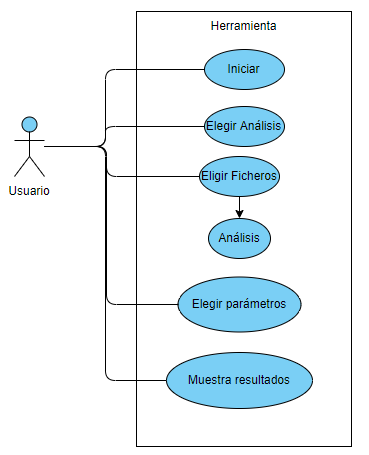
\includegraphics[width=10cm, height=8cm]{Uso}
\caption{Diagrama de casos de uso}
\end{figure}

